\documentclass[aspectratio=169,hyperref={pdfpagelabels=false}]{beamer}
\input{preamble.tex}
\usepackage{tikz}
\usepackage[siunitx]{circuitikz}
\usepackage{bm}
\usepackage{amsmath}
\usepackage{minted}
\usepackage{mathrsfs}

\usetikzlibrary{shapes.geometric, arrows, positioning}

\subtitle{\normalsize{Industrial IoT for Digitization of Electronis Assets}}
\title{Digital Twins, Models, and Parameters Estimation}

\setdepartment{DTU Wind and Energy System}
\setcolor{blue}

\begin{document}
\inserttitlepage

%SLIDE 0
\begin{frame}{Agenda}
  \begin{itemize}
    \item White, Grey, and Black Box Models
    \item LTI system and properties
    \item Autoregressive Model in System Identification
    \item Autoregressive with eXogenous 
    \item Parameters Estimation
    \item Examples in Python 
    \item Validation and Residual Analysis
    \item Order Selection
    \item AI \& ML in System Identification
  \end{itemize}
\end{frame}

% SLIDE 1
\begin{frame}{Model Types}
  \begin{figure}[t]
    \centering
    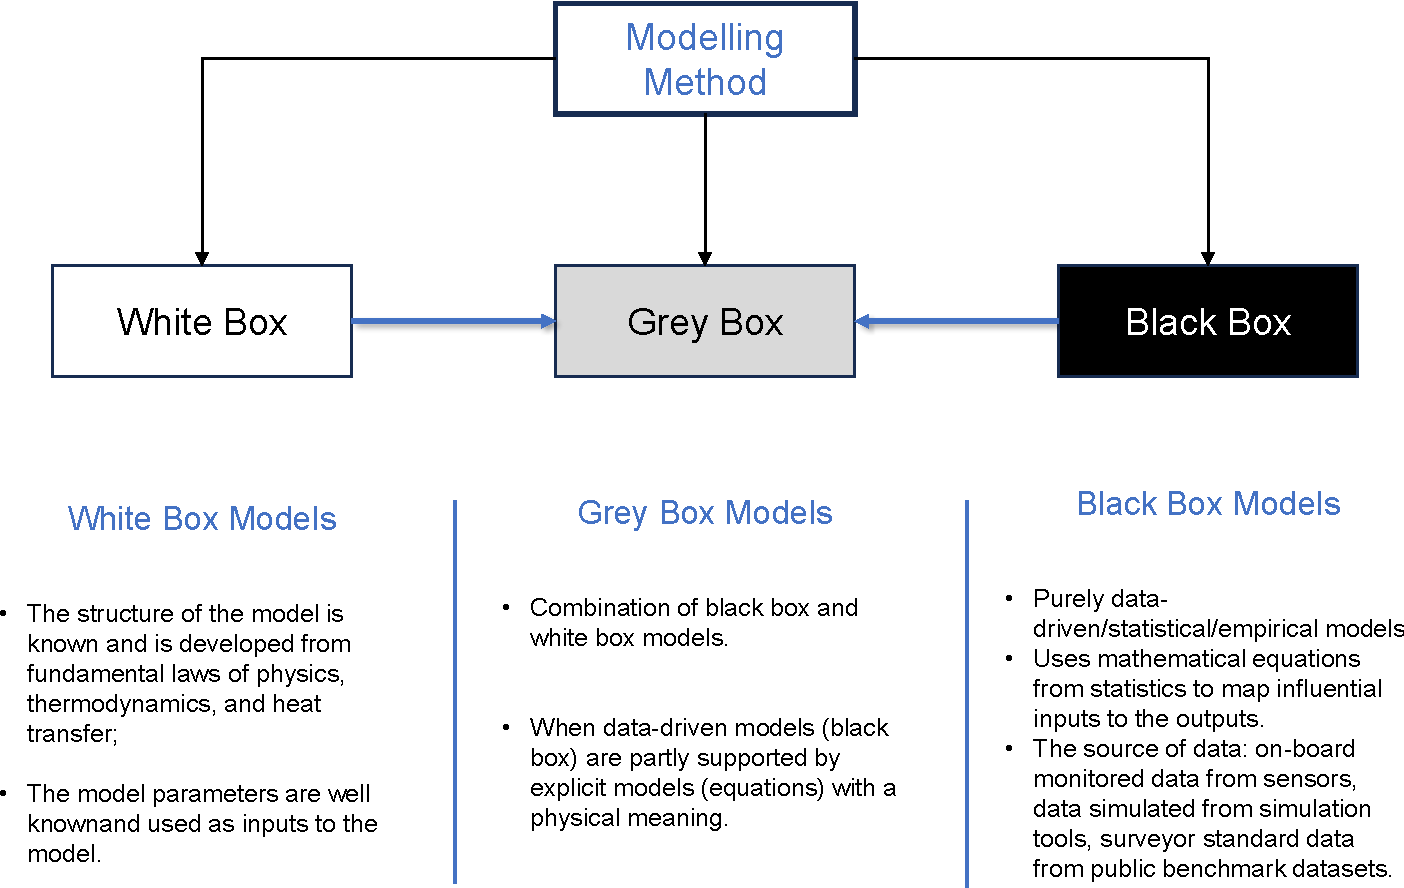
\includegraphics[width=0.85\textwidth]{img/modelling_methods.pdf}
\end{figure}
\end{frame}

% SLIDE 2
\begin{frame}{Example of White Box Model}
  Using the Kirchhoff's laws,
  we can write the equations: 
  \begin{columns}
    \begin{column}{0.4\textwidth}
      \begin{circuitikz}
        \draw
        (0,0) -- (0,1)
        (0,3) -- (0,2)
        to[open] (0,3) % Open circuit (gap) instead of voltage source
        to[R, l=$R_0$] (2,3) -- (4,3)
        to[R, l=$R_1$] (4,0) -- (0,0)
        (2,3) -- (2,2)
        (2,2) -- (2,3)
        to[C, l=$C$] (2,0);
        \node at (0.7,0.6) {{\small\textit{$t>0$}}};
    
        \draw(0,1) -- (0,1.2);
        \node at (-0.4,1.9) {$+$};
        \node at (-0.4,1.4) {$V$};
        \node at (-0.4,0.9) {$-$};
        %\draw[->,thick] (0.5,0.9) to[bend right] (0,1.5);
        %\node at (0.7,0.6) {{\small\textit{$t>0$}}};
    \end{circuitikz}
  \end{column}
  \begin{column}{0.6\textwidth}

  \begin{tcolorbox}[width=1\linewidth, height = 0.4\linewidth]
    \centering
    \begin{align*}
      I &= \frac{1}{R_1}V_{C} + C\frac{d}{dt}V_{C} \\
      V &= R_{0}I+ V_{C}\\
    \end{align*}
  \end{tcolorbox} \pause 
   
    \begin{tcolorbox}[width=1\linewidth, height = 0.3\linewidth]
      \centering
      \begin{align*}
        V + CR_{1}\frac{d}{dt}V = (R_0 + R_1)I + CR_{0}R_{1}\frac{d}{dt}I
      \end{align*}
    \end{tcolorbox}
  \end{column}
  \end{columns}
  \let\thefootnote\relax\footnotetext{\tiny{Willems, J. C., \& Polderman, J. W. (1997). Introduction to mathematical systems theory: a behavioral approach (Vol. 26). Springer Science \& Business Media.}}
\end{frame}

% SLIDE 3
\begin{frame}{Example of White Box Model}
  At time $t < 0$, the circuit is shorted ($V=0$) and at $t=0$ a $1V$ battery is attached.
  \begin{columns}
    \begin{column}{0.4\textwidth}
      \begin{circuitikz}
        \draw
        (0,0) -- (0,1)
        (0,3) -- (0,2)
        (0,0) to[battery] (0,3) % Open circuit (gap) instead of voltage source
        to[R, l=$R_0$] (2,3) -- (4,3)
        to[R, l=$R_1$] (4,0) -- (0,0)
        (2,3) -- (2,2)
        (2,2) -- (2,3)
        to[C, l=$C$] (2,0);
    
        \draw(0,1) -- (0,1.);
        \node at (-0.8,1.9) {$+$};
        \node at (-0.8,1.4) {$V$};
        \node at (-0.8,0.9) {$-$};
        %\draw[->,thick] (0.5,0.9) to[bend right] (0,1.5);
        %\node at (0.7,0.6) {{\small\textit{$t>0$}}};
    \end{circuitikz}
  \end{column}
\begin{column}{0.6\textwidth}

    \begin{figure}
      \centering
    
      \subfloat[Voltage step function.]{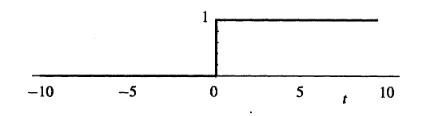
\includegraphics[width=0.8\textwidth]{img/pic9.png}}\\
      \subfloat[The current response.]{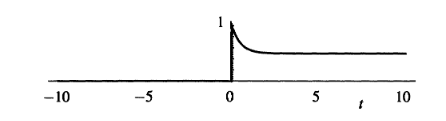
\includegraphics[width=0.8\textwidth]{img/pic8.png}}  
    \end{figure}
  \end{column}
  \end{columns}
\let\thefootnote\relax\footnotetext{\tiny{Willems, J. C., \& Polderman, J. W. (1997). Introduction to mathematical systems theory: a behavioral approach (Vol. 26). Springer Science \& Business Media.}}
\end{frame}

% SLIDE 4
\begin{frame}{Example of Grey Box Model}
  \begin{columns}
    \begin{column}{0.5\textwidth}
      \begin{tcolorbox}[width=1\linewidth, height = 1\linewidth]
      \textbf{Stochastic Models}
      \begin{align*}
        dx_t &= f(x_t, u_t, t, \theta) + \sigma(u_t, t, \theta)dw \\
        y_k  &= h(x_k, u_k, t_k, \theta) + e_k
      \end{align*}
    
      Suitable for both linear and non-linear models.  
      Used to represent systems influenced by both deterministic and stochastic components,
      accounting for random fluctuations in the system and uncertainties. \\
      \end{tcolorbox}\pause 

    \end{column}
    \begin{column}{0.5\textwidth}
      \begin{tcolorbox}[width=1\linewidth, height = 1\linewidth]
        \textbf{PINNs:Physics-informed neural networks} \\
        A class of machine learning techniques that combine data-driven neural
        networks with physical equations to solve complex problems in various fields,
        such as physics, and engineering, minimizing the discrepancy between the predictions made by the neural network and physical equations.
        \end{tcolorbox}
    \end{column}
\end{columns} 
\end{frame}

% SLIDE 5
\begin{frame}{Example of Black Box Models}
  A black box model is a system or algorithm that makes predictions or decisions based solely on input and output data,
  without an interpretable framework that can explain the connection between the inputs and the outputs.
  \begin{figure}
    \centering
    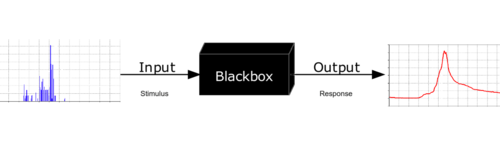
\includegraphics[scale=0.5]{img/pic10.png}
  \end{figure}
\end{frame}

% SLIDE 6
\begin{frame}{Definition of Dynamical System}
  \begin{block}{}
    A dynamical system $\Sigma$ is defined as a triple
  \[
    \Sigma = (T, W, \mathscr{B}),
  \]
  \begin{itemize}
    \item $T$ a subset of $\mathbb{Z}_+$ (in \textit{discrete-time systems}).
    \item $W$ a set called the \textit{signal space}.
    \item $\mathscr{B}$ a subset of $W^T$ called the \textit{behavior}.
  \end{itemize}
  \end{block}
  \let\thefootnote\relax\footnotetext{\tiny{Willems, J. C., \& Polderman, J. W. (1997). Introduction to mathematical systems theory: a behavioral approach (Vol. 26). Springer Science \& Business Media.}}
\end{frame}

% SLIDE 7 
\begin{frame}{Linear Time-Invariant (LTI) Dynamic Systems}
  \begin{block}{Definition:}
    \begin{itemize}
      \item[] A \textit{Linear Time-Invariant} (LTI) system is a dynamical system where the principles of superposition (linearity) and shift invariance (time invariance) hold.
    \end{itemize}
  \end{block}\pause

\begin{block}{Properties:}
  \begin{itemize}
    \item \textbf{Linearity:} Given $y_1(t)$ and $y_2(t)$ the outputs corresponding to inputs $x_1(t)$ and $x_2(t)$, then for any constants $a$ and $b$, the system's response to $ax_1(t) + bx_2(t)$ is $ay_1(t) + by_2(t)$.
    \item \textbf{Time Invariance:} If the output of the system to an input $x(t)$ is $y(t)$, then the output to an input $x(t - t_0)$, for any time shift $t_0$, is $y(t - t_0)$.
  \end{itemize}
\end{block}
\end{frame}

% SLIDE 8
\begin{frame}{AutoRegressive Model (\textbf{AR})}
  \begin{block}{First Order Model}
    Let's consider the simplest form of an AR model:
    \begin{equation*}
      y(t) = a_1 y(t-1) + \epsilon
    \end{equation*}
  \end{block}
    Where $\bm{y_{t-1}}$ is the \textit{lag} of $\bm{y}$ at time $t-1$ and $\bm{\epsilon}$ an error term. 
    \begin{block}{$\bm{n_a}$ order model}
      \begin{equation*}
        y(t) = {a}_{1}y(t-1) + a_{2}y(t-2) + \dots + a_{n_a}y(t-n_a) + \epsilon_t
      \end{equation*}
    \end{block}
  \end{frame}

% SLIDE 9
\begin{frame}{AutoRegressive eXogenous Model (\textbf{ARX})}
  \begin{block}{}
    Given an \textbf{LTI} system, with $\bm{y_t}$ the output signal \textit{with exogenous} input $\bm{u_t}$ with delay \textit{k}, an ARX model can be defined as follows:
    \begin{align*}
      y(t) = c + a_{1}y(t-1) + \dots + a_{n_a}y(t-n_a) + \\ 
              + b_{1}u(t-n_k) + \dots + b_{n_b}u(t-n_k-n_b-1) + \epsilon(t)      
    \end{align*}
    \begin{itemize}
      \item $\bm{n_a}$: numbers of lags of the output signal $y$.
      \item $\bm{n_b}$: numbers of lags of input signal $u$.
      \item $\bm{n_k}$: delay order between the $y$ and $u$.
    \end{itemize}
     
    \begin{align*}
      \boxed{y(t) = \varphi'\theta + \epsilon(t)}
    \end{align*}
  \end{block}
  \end{frame}

% SLIDE 10
  \begin{frame}{AutoRegressive eXogenous Model (\textbf{ARX})}
    \begin{block}{}
      Or equivalently:
      \vspace{0.1em}
      \begin{align*}
        \boxed{y(t) = \varphi'\theta + \epsilon(t)}
      \end{align*}
    \begin{align*}
      \bm{\theta} &= [a_1, \dots, a_{n_a} \; b_1, \dots, b_{n_b}]' \hspace{0.5em }\textit{\textcolor{red}{unknown parameters}} \\
      \bm{\varphi}(t) &= [y(t-1), \dots, y(t-n_a) \; u(t-n_k) \dots, u_{t-n_k-n_b+1}]' \hspace{0.5em }\textit{\textcolor{red}{regressors}}\\
      \bm{\epsilon}(t) &\sim \mathcal{N}(0,\sigma^2) \hspace{0.5em }\textit{\textcolor{red}{error}}
    \end{align*} \pause  
    \end{block}
    \end{frame}

% SLIDE 11
\begin{frame}{}
  \begin{block}{Remark}
    We denote $\bm{\hat{y}(t|\theta) = \varphi(t)'\theta}$ the estimated output prediction
  to emphasize that the estimate of $\hat{y}$ depends on the past data and the parameters vector $\theta$ with $\epsilon=0$ (best case scenario - \textbf{no residual error}).
  \end{block}\pause
  
  \vspace{2em}  
  \begin{columns}
    \column{0.4\textwidth} 
     
\includegraphics[width=0.7\textwidth]{img/pic5.png} \centering \pause
    \column{0.5\textwidth} % Second column
    \begin{itemize}
      \item $\bm{\varphi}' \rightarrow$ regressor vector (past data)
      \item $\bm{\epsilon(t)} = 0 \rightarrow $ (known distribution)
      \item[] \vspace{2em} \hspace{2em}\textbf{What is still missing?}   \pause
    \end{itemize}
    \end{columns}
\end{frame}

% SLIDE 12
\begin{frame}{}
  \begin{block}{Remark}
    We denote $\bm{\hat{y}(t|\theta) = \varphi(t)'\theta}$ the estimated output prediction
  to emphasize that the estimate of $\hat{y}$ depends from the past data on the parameters vector $\theta$ with $\epsilon=0$ (best case scenario - \textbf{no residual error}).
  \end{block}
  
  \vspace{2em}  
  \begin{columns}
    \column{0.4\textwidth} 
     
\includegraphics[width=0.7\textwidth]{img/pic5.png} \centering
    \column{0.5\textwidth} % Second column
    \begin{itemize}
      \item $\bm{\varphi}' \rightarrow$ regressors vector (past data)
      \item $\bm{\bar{\epsilon}} = 0 \rightarrow $ (known distribution)
      \item {$\bm{\theta}$ is the coefficients vector (to be estimated)}
    \end{itemize}
    \end{columns}
\end{frame}

% SLIDE 13
\begin{frame}{Parameters Estimation}
      \begin{block}{}
        We don't know $\theta$ yet, but we have collected a set $Z^N$ of measured data.
        \begin{align*}
          Z^N = \{u(-n), y(-n)\dots u(N-1), y(N-1) \}, \: n = max\{n_a,n_{b}+n_{k}-1\}
        \end{align*}
      Therefore, we use the \textcolor{red}{least squared error} to find the optimal parameters vector $\theta^*$ that minimize the prediction error between $\hat{y}(t+1|\theta)$ and $y(t)$, namely: 
      \begin{align*}
        \theta^* = \underset{\theta}{\text{arg\;min}} \{\mathcal{L}(\theta, Z^N)\}
      \end{align*}
      \begin{align*}
        \mathcal{L}(\theta, Z^N) = \sum_{k=0}^{N-1}(y(t)-\hat{y}(t|\theta))^2 = \sum_{k=0}^{N-1}(y(t)-\varphi'(t)\theta)^2 
      \end{align*}
    \end{block}
\end{frame}

% SLIDE 12
\begin{frame}{Paramters Estimation}
  \begin{block}{}
      $\mathcal{L}(\theta, Z^N)$ is a quadratic function of $\theta$. Therefore, $\theta^*$ can be found by zeroing The derivative of $\mathcal{L}$.
  \begin{align*}
    \frac{d}{d\theta} \mathcal{L}_N(\theta, Z^N) = 2\sum_{k=0}^{N-1}\varphi(t)(y(t)-\varphi'(t)\theta)  = 0 
  \end{align*}
Thus, obtaining: 
\begin{align*}
  \sum_{k=0}^{N-1}\varphi(t)y(t) = \sum_{k=0}^{N-1}\varphi(t)\varphi'(t)\theta
\end{align*}
Finally, the $\theta^*$ can be derived: 
\begin{center}
    \begin{align*}
      \boxed{\theta^* = \Biggr[\sum_{k=0}^{N-1}\varphi(t)\varphi'(t)\Biggr]^{-1} \: \Biggr[\sum_{k=0}^{N-1}\varphi(t)y(t)\Biggr]}
    \end{align*}
\end{center}
\end{block}
\end{frame}

% SLIDE 13
\begin{frame}{Paramters Estimation}
  \begin{block}{}
    Thus, obtaining: 
\begin{align*}
  \sum_{k=0}^{N-1}\varphi(t)y(k) = \sum_{k=0}^{N-1}\varphi(t)\varphi'(k)\theta
\end{align*}
Finally, $\theta^*$ can be derived: 
\begin{center}
\begin{tcolorbox}[width=0.6\linewidth, height = 0.22\linewidth, colframe=red]
    \begin{align*}
      \theta^* = \Biggr[\sum_{k=0}^{N-1}\varphi(t)\varphi'(t)\Biggr]^{-1} \: \Biggr[\sum_{k=0}^{N-1}\varphi(t)y(t)\Biggr]
    \end{align*}
\end{tcolorbox}
\end{center}
\end{block}
\end{frame}

% SLIDE 22
\begin{frame}[fragile]{}
  \begin{columns}[T]

    \begin{column}{.33\textwidth}
    \begin{block}{MAE (Mean Absolute Error)}
    The MAE is the average of the absolute errors between prediction \(\hat{y}_i\)  and actual observations \(y_i\). It's calculated as:
    \begin{equation*}
      \text{MAE} = \frac{1}{n} \sum_{i=1}^n |y_i - \hat{y}_i|
    \end{equation*}
    \vspace{0.4em}
    \end{block}
    \end{column}
    
    \begin{column}{.33\textwidth}
    \begin{block}{RMSE (Root Mean Square Error)}
    The RMSE is the square root of the average of squared differences between prediction \(\hat{y}_i\) and actual observation \(y_i\). It's calculated as:
    \begin{equation*}
      \resizebox{\columnwidth}{!}{$\text{RMSE} = \sqrt{\frac{1}{n} \sum_{i=1}^n (y_i - \hat{y}_i)^2}$}
    \end{equation*}
    \vspace{0em}
    \end{block}
    \end{column}
    
    \begin{column}{.33\textwidth}
    \begin{block}{RRMSE (Relative Root Mean Square Error)}
    RRMSE is the RMSE normalized against the actual value measurement \(\hat{y}_i\).
    \begin{equation*}
      \resizebox{\columnwidth}{!}{$\text{RMSE} = \sqrt{\frac{\frac{1}{n} \sum_{i=1}^n (y_i - \hat{y}_i)^2}{\sum_{i=1}^n(\hat{y}^)2}}$}
    \end{equation*}
    \vspace{1.8em}
    \end{block}
    \end{column}
    
    \end{columns}
\end{frame}

% SLIDE 23
\begin{frame}{}
  \begin{columns}
  \column{0.3\textwidth} 
  
\includegraphics[width=0.6\textwidth]{img/pic5.png} \centering
  
  \column{0.7\textwidth} % Second column
    \textbf{Do you rember the assumtion on} $\epsilon(t)$ \textbf{?} \centering \\
    \vspace{2em}
    We previously assumed that the residual of the model, namely $(y - \hat{y})$ 
    are distributed as $\epsilon(t)\sim \mathcal{N}(0,\sigma^2)$.
    \vspace{2em}

    In our example we have introduce a distrurbance modeled as gaussian noise with $\sigma = 0.1$
    If the model is good enough, we error will coincide with the gaussian noise we introduced.
  \end{columns}
\end{frame}

% SLIDE 24
\begin{frame}{Model Validation}
  \textbf{Shapiro-Wilk} test confirmed that the residuals are white noise and the Q-Q Plot below shows that the distribution of the residual is compatible with the noise introduced in our data $\sim \mathcal{N}(0,\sigma^2 = 0.1)$.
  \begin{figure}
    \centering
    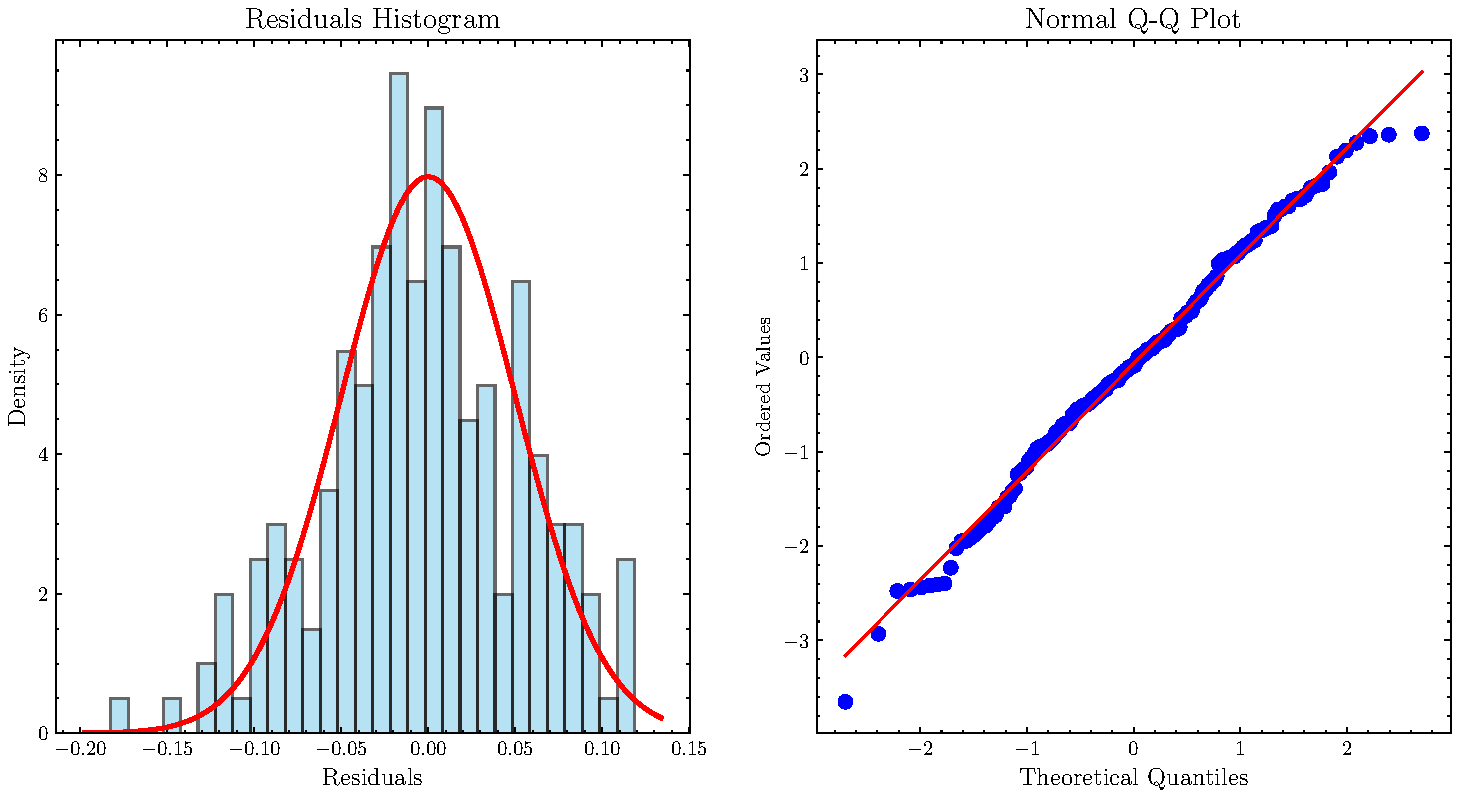
\includegraphics[width=0.7\linewidth]{img/residuals_analysis.pdf}
  \end{figure}
\end{frame}

\begin{frame}
  \frametitle{Model Selection: \textit{AIC} \& \textit{BIC}}

  AIC and BIC are fundamental statistical tools used to select the best model from a group of potential models based on their performance with a given dataset. 
  They are particularly crucial when there are multiple models, as they help balance fitting the data and model complexity, thus preventing overfitting or underfitting.
\end{frame}


\begin{frame}
  \frametitle{Model Selection: \textit{AIC} \& \textit{BIC}}
  \begin{columns}
    \begin{column}{0.5\textwidth}
      \begin{block}{Akaike Information Criterion (AIC)}
        \textbf{Definition:} 
        \begin{align*}
          \boxed{\text{AIC} = 2k - 2\ln(L)}
        \end{align*}
          where: 
        \begin{itemize}
          \item \textbf{k} is the number of parameters
          \item \textbf{L} is the maximum likelihood of the model.
        \end{itemize}
        \vspace{1.5em}
      \end{block}
    \end{column}
    
    \begin{column}{0.5\textwidth}
      \begin{block}{Bayesian Information Criterion (BIC)}
        \textbf{Definition:}
        \begin{align*}
          \boxed{\text{BIC} = \ln(n)k - 2\ln(L)}
        \end{align*} 
        where: 
        \begin{itemize}
          \item  \textbf{n} is the number of observations
          \item \textbf{k} is the number of parameters
          \item \textbf{L} is the maximum likelihood of the model.
          
        \end{itemize}
      \end{block}
    \end{column}
  \end{columns}
\end{frame}


\begin{frame}
  \frametitle{Model Selection: \textit{AIC} \& \textit{BIC}}
  \begin{columns}
    \begin{column}{0.5\textwidth}
      \begin{block}{Akaike Information Criterion (AIC)}
        \textbf{Definition:} 
        \begin{itemize}
          \item Balances model fit and complexity.
          \item More emphasis on goodness of fit than on simplicity.
            \item [] \textbf{Limitations:}
            \item Relative measure; cannot be used to test a single model.
            \item Can be biased in small samples.
        \end{itemize}
      \end{block}
    \end{column}
    
    \begin{column}{0.5\textwidth}
      \begin{block}{Bayesian Information Criterion (BIC)}
        \textbf{Definition:}
        \begin{itemize}
          \item Includes a penalty term for the number of observations
          \item making it more reliable for larger datasets.
          \item Favors simpler models compared to AIC.
          \item Assumes that the model errors are independently and identically distributed.
        \end{itemize}
      \end{block}
    \end{column}
  \end{columns}
\end{frame}

\begin{frame}{Likelihood Function}
  \begin{definition}
      The likelihood function measures the probability of observing the given data under different parameter values of a statistical model.
  \end{definition}
  
  \begin{equation*}
      L(\theta | x) = P(X = x | \theta)
  \end{equation*}
  
  \begin{itemize}
      \item $\theta$: Parameters of the model
      \item $x$: Observed data
      \item $L(\theta | x)$: Likelihood of parameter $\theta$ given data $x$
  \end{itemize}

\end{frame}


\end{document}